%%%%%%%%%%%%%%%%%%%%%%%%%%%%%%%

%\fixme{KM: done for now, but am not satisfied with the end of it-- Juergen did not provide measurements! SG/JM: please briefly check to make sure it is coherent? SG: done. Sent an email to Juergen with some items to be addressed.}

%\subsubsection{Physics Motivation}

Radioactive source deployment provides an in-situ source of physics signals at a known location and with a known activity that can be chosen such that there is only one calibration event per drift time window. The 
primary
%baseline 
source design probes de-excitation products ($\gamma$-rays) which are directly relevant for detection of supernova neutrinos and \isotope{B}{8}/hep solar neutrinos. The \dlong{rsds} (\dshort{rsds}) is the only calibration system that could probe the detection capability for single isolated solar neutrino events and study how well radiological backgrounds can be suppressed. The trigger efficiency could be studied as a function of threshold. 

Other measurements with the primary source include electro-magnetic (EM) shower characterization for long-baseline $\nu_e$ CC events, electron lifetime and electric field as a function of \dword{detmodule} vertical position, individual light detector response, and determination of radiative components of the Michel electron energy spectrum from muon decays. Aside from the 
%baseline
primary nickel source that produces \SI{9}{\MeV} $\gamma$-rays via the \isotope{Ni}{58}(n,$\gamma$)\isotope{Ni}{59} reaction, other sources could be deployed with the same multi-purpose system, for example an ($\alpha$,$\gamma$)
 %\isotope{Ar}{40}($\alpha$,$\gamma$)\isotope{Ca}{44}
%\fixme{isn't this actually an alpha source?}
%gamma-ray 
source, and \isotope{Cf}{252} and/or AmBe neutron sources that probe the impact of various radiological backgrounds, like radon (causing  ($\alpha,\,\gamma$) events) or radiological neutrons, or simply measure the neutron tagging efficiency, useful for improved calorimetry of beam neutrino interactions. In contrast to the primary %$^{58}$Ni(n,$\gamma$)$^{59}$Ni
nickel source with \SI{9}{\MeV} gamma-rays, the ($\alpha$,$\gamma$) source producing gamma-ray energies around \SI{15}{\MeV} via the
\isotope{Ar}{40}($\alpha$,$\gamma$)\isotope{Ca}{44}
%$^{40}Ar(\alpha,\,\gamma)^{44}$Ca 
reaction could even be deployed outside of the cryostat, to probe the upper visible energy range and trigger efficiency for \isotope{B}{8}/hep solar neutrinos. 

Both the \dshort{rsds} and the \dword{pns} systems are needed to address the integrated response of the detector for low energy physics, especially \dword{snb} and $^{8}B$/hep solar neutrinos. 
The \dword{rsds} primarily probes for trigger efficiency, the \dword{pns} tests mostly for uniformity. Response in argon may change rapidly as a function of photon energy due to underlying nuclear physics mechanisms. A combination of \SI{6}{\MeV} (direct neutron capture response), \SI{9}{\MeV} (from the nickel source),
%(peak visible $\gamma$-energy of interest to \dword{snb} and $^{8}B$/hep solar neutrinos), 
\SI{15}{\MeV} (from the ($\alpha$,$\gamma$) source)
is needed to map the low energy response. In terms of complementarity, radioactive sources provide a known position, known-energy single photon events that could be triggered on, while the pulsed neutron source provides a simple, potentially, non-invasive design with externally triggered multi-photon energy signature which is visible across the entire detector with a known time signature.


%%%%%%%%%%%%%%%%
\subsubsection{Design Considerations}

A composite source can be used that consists of \isotope{Cf}{252}, a strong neutron emitter, and \isotope{Ni}{58}, which, via the \isotope{Ni}{58}(n,$\gamma$)\isotope{Ni}{59} process, converts one of the 
\isotope{Cf}{252} fission neutrons, suitably moderated, to a monoenergetic \SI{9}{\MeV} photon~\cite{Rogers:1996ks}. 
The source is envisaged to be inside a cylindrical moderator with mass of about \SI{15}{\kg} and a diameter of \SI{20}{\cm} such that it can be deployed via the multipurpose instrumentation ports discussed in Section~\ref{sec:sp-calib-cryostat}. The activity of the radioactive source is chosen such that no more than one \SI{9}{\MeV} capture $\gamma$-event occurs during a single drift period. This forms the main requirement for this system as this allows one to use the arrival time of the measured light as a $t_0$ and then measure the average drift time of the corresponding charge signal(s). Table~\ref{tab:fdgen-calib-all-reqs-rsds} lists the full set of requirements for the \dlong{rsds}.

The sources would be deployed outside the \dword{fc} within the cryostat to avoid regions with a high electric field, about \SI{30}{\cm} from the field cage. The $\gamma$-ray would need to travel about two attenuation lengths (including the \SI{10}{\cm} radius of the source body). Such high $\gamma$-energies are typically only achieved by thermal neutron capture, which invokes a neutron source surrounded by a large amount of moderator, thus driving the size of the source.
%making such an externally deployed (n, $\gamma$) source \SI{20}{\cm}  to \SI{50}{\cm} % large
%in diameter. 

\begin{dunetable}
[Full specifications for the radioactive source deployment system]
{p{0.45\linewidth}p{0.25\linewidth}p{0.25\linewidth}}
{tab:fdgen-calib-all-reqs-rsds}
{Full list of Specifications for radioactive source deployment system.}   
Quantity/Parameter	& Specification	& Goal		 \\ \toprowrule   
%\textbf{Proposed Radioactive Source System}	   &   &  \\ \colhline  
Distance of the source from the field cage & \SI{30}{\cm} & \\ \colhline
Rate of \SI{9}{\MeV} capture $\gamma$-events inside the source {(\it top-level requirement)} & < \SI{1}{\k\hertz} & \\ \colhline 
Data volume per \SI{10}{\kt}  & \SI{50}{\TB\per\year} & \SI{100}{\TB\per\year} \\ \colhline 
Longevity	& \dunelifetime			& > \dunelifetime   \\     
%Stability & Match precision requirement at all places/times	&  \\ \colhline  Reliability	& Measurements as needed & Measurements as needed \\ \colhline

\end{dunetable}

%In~\cite{Rogers:1996ks}, %\fixme{This needs to be restated: In Jones [4]... (with Jones being the name of the author).}
%\cite{Triumf:Nickelsource} 
%\todo{SG: reference needs fixing},
A gamma source based on the \isotope{Ni}{58}(n,$\gamma$)\isotope{Ni}{59} reaction, and triggered by an AmBe neutron source, has been successfully built~\cite{Rogers:1996ks}, yielding high $\gamma$-energies of \SI{9}{\MeV}. DUNE %We 
proposes to use a \isotope{Cf}{252} (or AmLi as backup) neutron source with lower neutron energies, which requires less than half of the surrounding moderator, and making the \isotope{Ni}{58} (n, $\gamma$) source only \SI{20}{\cm} or less in diameter. The multipurpose instrumentation feedthroughs at either end of the cryostat are sufficient for this, and have an outer diameter of \SI{25}{\cm}.  The moderator material chosen for DUNE is Delrin,\footnote{DuPont\texttrademark Delrin\textregistered, \url{http://www.dupont.com/products-and-services/plastics-polymers-resins/thermoplastics/brands/delrin-acetal-resin.html}.} which has a large enough density to avoid flotation. Further, the end caps of the source body are round to avoid distorting the electric field and to eliminate the risk of the source getting stuck during deployment. 
Figure~\ref{fig:RadioactiveSource_zm40cm_xp220cm} depicts the primary source design of a cylindrical Delrin moderator with a diameter of \SI{20}{\cm}, a height of \SI{40}{\cm} including half-spheres at either end with radius of \SI{10}{\cm}, deployed at $z$=\SI{40}{\cm} leaving a gap of \SI{30}{\cm} towards the \dword{fc} and at a distance to the \dword{apa} of $x$=\SI{220}{\cm}, which is slightly further than mid-drift.

\begin{dunefigure}[Fish-line deployment scheme in \dshort{dune} for an encapsulated radioactive source]{fig:RadioactiveSource_zm40cm_xp220cm}{Fish-line deployment scheme in \dword{dune} for a radioactive source encapsulated inside a cylindrical Delrin moderator body \SI{20}{\cm} in diameter and \SI{40}{\cm} high, including half-spheres with a radius of \SI{10}{\cm} at either end. A \isotope{Cf}{252} neutron source and a natural Ni target are sealed inside at the center. The fish-line is deployed \SI{40}{\cm} outside of the \dword{fc} and \SI{220}{\cm} away from the \dword{apa} (red plane).}
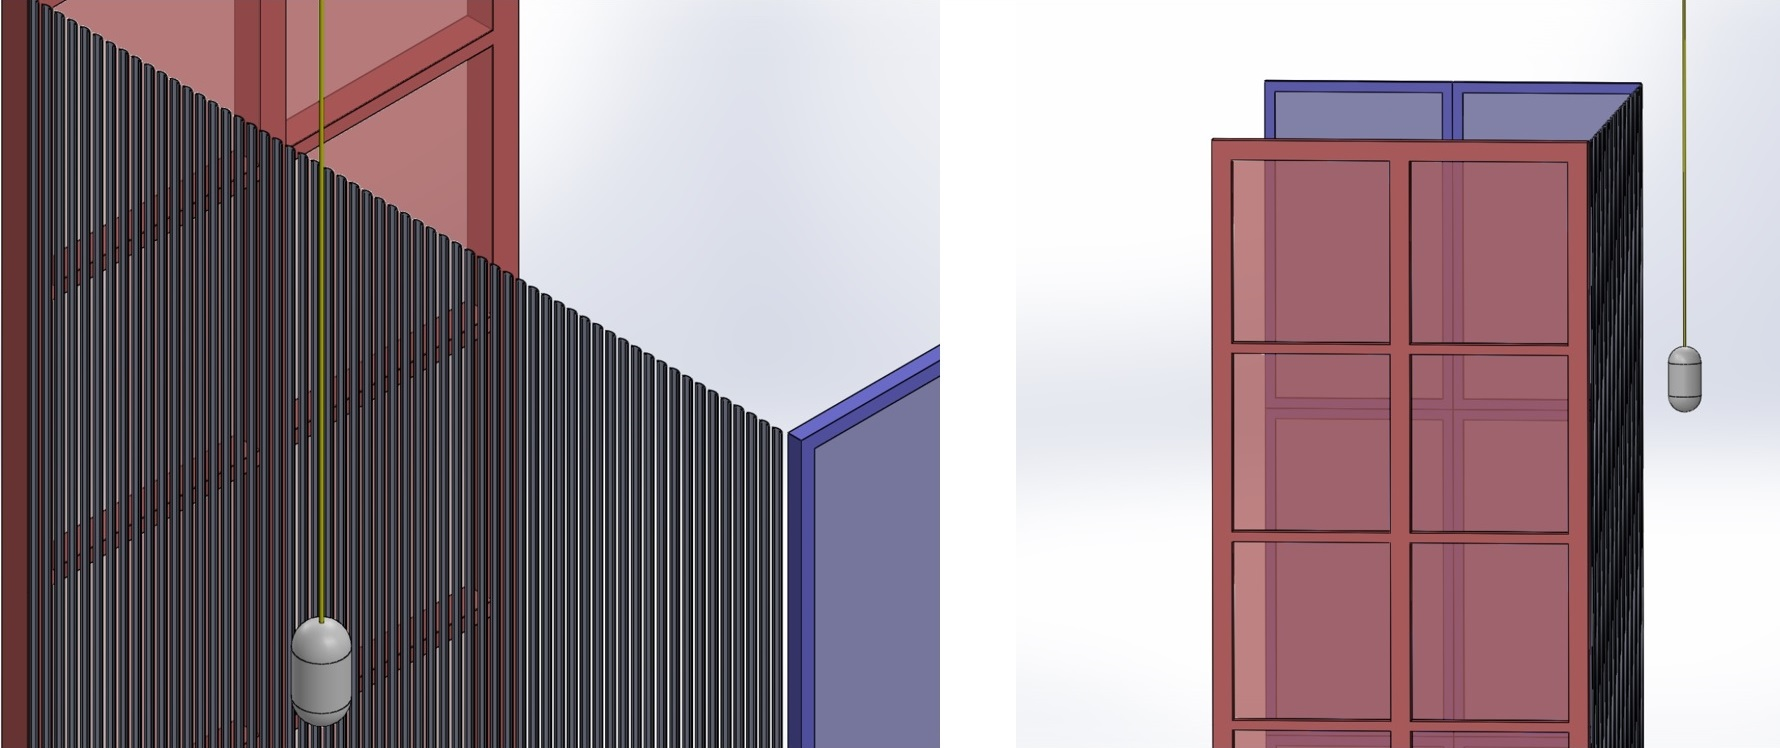
\includegraphics[width=1.0\linewidth]{RadioactiveSource_zm40cm_xp220cm.jpg}
\end{dunefigure}

% Here it is, but I don't have privileges for the bibliography

%@Misc{Triumf:Nickelsource,
%  author =   {J. Rogers, M. Andreaco, C. Moisan},
%  title =    {A $7-9$\,MeV isotropic gamma ray source for detector testing},
%  howpublished = {TRIUMF TRI-PP-96-7},
%  month =    {Apr},
%  year =     {1996},
%}

%\fixme{KM: From Juergen but I think covered by above: The activity of the radioactive source is chosen such that no more than one \SI{9}{\MeV} capture $\gamma$-ray spills into the active \dword{lartpc} region during a single \SI{2.2}{\milli\s} drift period. This allows one to use the arrival time of the measured light as $t_{0}$ and then measure the average drift time of the corresponding charge signal(s). The resulting drift velocity in turn yields the electric field strength, averaged over the variations encountered during the drifting of the charge(s). This can be repeated for each single \SI{9}{\MeV} capture $\gamma$-event that occurs during a \SI{2.2}{\milli\s} drift period and where visible $\gamma$-energy is deposited inside the active volume of the TPC. Pile-up and data read-out considerations restrict the maximally permissible event rate to less than \SI{10}{\hertz} and in turn the \SI{9}{\MeV} capture $\gamma$-rate occurring inside the radioactive source body to less than \SI{140}{\hertz}, given a spill-in efficiency into the active \dword{lar} of about \num{7}\%.}

A successfully employed multipurpose fish-line calibration
system
%~\cite{bib:deKerret2012} \todo{SG: Juergen to provide proper reference. JM: Juergen says there's no alternative public ref.} 
% JM, April 2018: We will not refer to this since the LBNC will not have access to it
%\fixme{need to add reference: "The Double Chooz Near Detector Technical Design Report" 
%Double Chooz Collaboration (H. de Kerret (APC, Paris) et al.) Oct 1, 2012. EDMS ID:I-028812 ; DocDB ID: 3403-V5 Pages 198 - 223
%(Anne can't find proper ref for this)}
for the Double Chooz reactor neutrino experiment has become available 
 %for DUNE 
after the decommissioning of Double Chooz in 2018. The system can be easily refitted for use in \dword{dune}. The system will be housed inside a purge-box that is connected via a neck to a multipurpose calibration feedthrough with a closed gate valve on top of the cryostat. Before deployments, the source will be gently cooled-down by blowing liquid argon boil-off onto it inside a sealed purge-box. After the source has reached 
%near liquid argon 
near-\dword{lar} temperatures, the purge-box will be evacuated by a vacuum pump to remove any residual oxygen and nitrogen which is monitored at the ppm level. Then, the entire purge-box interior is purged with boil-off liquid argon, and the pressure equalized with the gas pressure inside the detector, before the gate-valve is opened and deployments can commence. This procedure ensures that no significant impurities are introduced into the detector during a deployment and that no significant amount of liquid argon is boiled-off from the detector. 
%Also, if the source is in close proximity of an \dword{apa} wire frame, lower energetic radiological backgrounds become problematic as the source light and charge yield is reduced exponentially with distance. 

Deployed near mid-drift (in each TPC module) the \SI{9}{\MeV} $\gamma$-ray source can illuminate the full drift length from \dword{apa} to \dword{cpa}. The sources are retrieved from the detector after each deployment and stored outside the cryostat following approved safety protocols, and the gate-valves are kept closed after deployments. More details on radiation safety and handling procedures are presented in Section~\ref{sec:sp-calib-rsds-safety}.

\subsubsection{Development Plan}
The major development plans for the \dlong{rsds} include
\begin{itemize}
\item Continued development of relevant simulation tools including geometry representation of the source deployment system and impact from various radiological contaminants on detector response. 
\item Studies to suppress radiological backgrounds for the calibration source.
\item Simulation studies to understand data and trigger rates.
\item A baseline design source with Delrin moderator, $^{252}$Cf neutron source, and natural nickel target, both sealed inside at the moderator's center.
\item Validation of \SI{9}{\MeV} capture $\gamma$-ray yield of source using spectroscopic measurements with the `RABBIT' germanium detector at South Dakota School of Mines and Technology (SDSMT), that has an assay chamber large enough to fit the bulky moderator. 
%\fixme{Check this please. SG: check what?}
\item Validation with $^{3}$He based hodoscope at SDSMT to ensure that the flux of neutrons escaping the moderator is not an issue; otherwise use lower energetic AmLi neutron source instead and/or more moderator material, and/or different geometric configuration of nickel target. 
\item Test gentle GAr cooling of source and validate material integrity. Measure tensile strength of braided SS-304 wire-rope at cryogenic temperatures and ensure a safety factor of one order of magnitude by adjusting number of steel braids and their diameters. Validate cryogenic shrinkage of sectional teflon sleeves, that enclose the braided steel wire-rope and electrically insulate it towards the \dword{fc}. 
\item Validation that anticipated fluid flow in \dword{lar} does not cause oscillations of the source; otherwise design vertical guide wires to be pre-installed during detector installation 
%and that they 
which will keep source in stable position during deployment along the vertical axis.
%\item A mechanical test of the Double Chooz fish-line deployment system with both an \dword{lar} and liquid nitrogen mock-up column in the high bay lab at South Dakota School of Mines and Technology. The ultimate test of the system will be done at ProtoDUNE. 
\item Explore other radioactive sources beyond the primary %$^{58}$Ni(n,$\gamma$)$^{59}$Ni 
\SI{9}{\MeV} $\gamma$-ray nickel source, such as the previously mentioned \SI{15}{\MeV} $\gamma$-ray source based on the  $^{40}$Ar($\alpha,\,\gamma$)$^{44}$Ca process with $^{241}$Am as the alpha emitter. This is currently being assembled at SDSMT.
%a non-invasive externally employed 
%with $^{241}$Am that is currently being assembled at SDSMT, and that could probe from the outside of the cryostat the upper visible energy range and trigger efficiency for $^{8}B$/hep solar neutrinos. 
Furthermore, investigate hybrid neutron sources ($^{252}$Cf and AmBe) that emulate the kinetic neutron energy spectrum of radiological neutrons and probe the neutron tagging efficiency.
%, useful for improved calorimetry of beam neutrino interactions and for clarification of impact of radiological neutron backgrounds. 
\end{itemize}

A successful demonstration of the \dword{rsds} in \dword{protodune2} running is the main priority for this system towards making a decision on deploying this system for the \dword{fd}. A schedule with main steps towards \dword{protodune2} deployment is shown in Table~\ref{tab:calib-rsds-sched}.

\begin{dunetable}
[Key milestones for commissioning RSDS in \dshort{protodune2}]
{p{0.65\textwidth}p{0.25\textwidth}}
{tab:calib-rsds-sched}
{Key milestones towards commissioning the \dlong{rsds} in \dword{protodune2}.}  
Milestone & Date (Month YYYY)   \\ \toprowrule
Baseline \dword{rsds} design validation & January 2020 \\ \colhline 
\dword{rsds} mock-up deployment test at SDSMT & March 2020 \\ \colhline 
\dword{rsds} Design review  & May 2020 \\ \colhline
\dword{rsds} Production readiness review (PRR) & July 2020 \\ \colhline
Start of module 0 \dword{rsds} component production for \dword{protodune2} & September 2020      \\ \colhline
End of module 0 \dword{rsds} component production for \dword{protodune2} &  February 2021    \\ \colhline
\textbf{Start of \dword{protodune2} (\single) installation} & \textbf{March 2021} \\ \colhline
Start of \dword{rsds} installation &  April 2021    \\ \colhline
\dword{rsds} demonstration test at \dword{protodune2}  & April 2022\\ 
\end{dunetable}

%%%%%%%%%%%%%%%%%%%%%%%%%%%%
\subsubsection{Measurement Program}
\label{sec:sp-calib-sys-src-dep-meas}

The proposed primary \SI{9}{\MeV} single $\gamma$ source may also be used to test the $\gamma$ component of the \dword{snb} and \isotope{B}{8}/hep solar neutrino signal along the full drift but only in the endwall regions of the detector. The source may also be used to determine the relative charge and light extraction efficiency in the vertical direction for measurements of energy resolution and energy scale. 

%SG: this is repetition
%The \dword{rsds} is the only calibration system that could probe the detection capability for single isolated solar neutrino events and study how well radiological backgrounds can be suppressed. 
Figure~\ref{fig:rsds-fig1}
%{fig:9MeVgamma_withBG_LArSoft_v08_14_00_hiLY_originCHARGEcollected_TopView}
depicts in a top view of the detector the simulated charge extraction efficiency for the 9~MeV $\gamma$-ray source deployed \SI{40}{\cm} outside of the \dword{fc}, near mid-drift i.e., \SI{220}{\cm} away from the \dword{apa} in the $x$ direction, in the presence of expected background before (a) and after (b) applying selection cuts. The selection cuts
are based on the amplitude and location of wire hits, and require a coincidence with a suitable signal in the \dword{pds}.
%discard each collection wire hit with less than \num{90}~ADCU, limit wire hits to be within the width of the outer \dword{apa}, use induction wire hits to discard collection wire hits occurring further than \SI{2.2}{\m} away from the deployment height, and requiring at least one occurrence per \SI{2.2}{\ms} drift-time window of a simultaneously extracted (\SI{50}{\ns} time window) number of photoelectrons of more than \num{40}~pes .
Figure~\ref{fig:rsds-fig1}(b)
%Figure~\ref{fig:9MeVgamma_withBG_LArSoft_v08_14_00_hiLY_originCHARGEcollected_TopView} (b) 
shows that the selection cuts can reject radiological backgrounds almost entirely, and that
%, such that almost pure \SI{9}{\MeV} gamma-ray events are selected. 
the \dword{rsds} should allow the study of the trigger efficiency for isolated solar neutrino events, and its threshold dependence.

%SG: already stated under physics motivation, no need to repeat
%Moreover, the small electronic pulses from 9~MeV gamma-ray induced charge and light collections can be utilized to better characterize electro-magnetic (EM) showers for long-baseline $\nu_e$ CC events, as well as to determine the radiative components of the Michel electron energy spectrum from muon decays. 
%Further secondary measurements from the baseline 9 MeV gamma-ray source deployment include measuring the electron lifetime and electric field as a function of \dword{detmodule} vertical position, as well as the individual light detector response. 

Figure~\ref{fig:rsds-fig2}
%{9MeVgamma_withBG_LArSoft_v08_14_00_hiLY_DriftTimesEfield_ChargeSpectrumElectronLifetime_cut} 
shows exemplary simulated %baseline 
\dword{rsds} measurements of the \efield strength (a) and of the electron lifetime (b), each for three different scenarios. The analysis is based on fitting the measured distribution of drift-time, i.e., the time difference between the \dword{pds} signal
%an extracted number of photoelectrons of more than 40~pes 
and the recorded hit times on collection wires, passing the selection cuts.
%, defines the plotted drift-times. Precise quantities can be extracted from fitting the measured drift-time distribution to the simulation. 

%or this, the simulated collection wire charge (before selection cuts) is re-weighted with respect to 
%(a) 
%the \efield strength, and 
%(b) 
%the electron lifetime, respectively. After each re-weighting of the simulation the selection cuts are then applied. 
Figure~\ref{fig:rsds-fig2}(a)
%{9MeVgamma_withBG_LArSoft_v08_14_00_hiLY_DriftTimesEfield_ChargeSpectrumElectronLifetime_cut} (a) 
illustrates that with this method the \efield strength could be measured at $\sim$ \SI{1}{\%} precision at each vertical deployment position at the endwalls. Likewise, Figure~\ref{fig:rsds-fig2}(b)
%Figure~\ref{9MeVgamma_withBG_LArSoft_v08_14_00_hiLY_DriftTimesEfield_ChargeSpectrumElectronLifetime_cut} (b) 
illustrates that the electron lifetime could be measured at about $\sim$ \SI{10}{\%} precision (possibly better at higher lifetimes) at each vertical deployment position at the endwalls. 

Figure~\ref{fig:rsds-fig2}(c)
%{9MeVgamma_withBG_LArSoft_v08_14_00_hiLY_DriftTimesEfield_ChargeSpectrumElectronLifetime_cut} (c) 
illustrates that it is not convincingly possible to unambiguously measure both the electron lifetime and the electric field strength with a recorded charge spectrum (after selection cuts) alone, since both parameters simply shift the upper falling edge of the charge spectrum up or down. However, when combined with the drift-time measurement, the charge measurement would provide an additional constrain that could possibly break correlations. 

%However, at each vertical \dword{rsds} deployment position at the endwalls, it is still possible to self-consistently measure both the electron lifetime and the electric field strength at $\sim 1\%$ precision: First, the electric field strength is precisely inferred from the drift-time distribution at each deployment position, second the corresponding electron lifetime is then precisely deduced from the charge distribution by using the measured electric field strength as precise constraint. 

%Figure~\ref{fig:rsds-fig2plus} visualizes the simulated change of individual light detector response as a function of \dword{detmodule} vertical position when the baseline source is deployed at one of the possible endwall locations. The uniformity of the optical detection response can be probed with a full vertical scan. Wrong channel mapping, dead or noisy optical detectors could be easily identified. 

Aside from the primary
%$^{58}$Ni(n,$\gamma$)$^{59}$Ni 
9 MeV $\gamma$-ray nickel source, other sources could be deployed with the same multi-purpose system, for example a $^{40}$Ar($\alpha,\,\gamma$)$^{44}$Ca gamma-ray source, a $^{252}$Cf and/or AmBe neutron source that probe the impact of various radiological backgrounds, like radon ($\alpha,\,\gamma$) or radiological neutrons, or simply measure the neutron tagging efficiency, useful for improved calorimetry of beam neutrino interactions. 
In contrast to the nickel source, the \SI{15}{\MeV} ($\alpha,\,\gamma$) could be deployed outside of the cryostat.
%and probing the upper visible energy range and trigger efficiency for $^{8}B$/hep solar neutrinos. 
%Figure~\ref{fig:rsds-fig3}
%{5MeValphaSource_zx_TDR_TopView} 
%shows in a top view of the detector the widely spread interaction locations of about half a dozen $^{40}Ar(\alpha,\,\gamma)^{44}$Ca 15 MeV $\gamma$-ray events in terms of detected light (Figure~\ref{fig:rsds-fig3}(a)) and  detected charge (Figure~\ref{fig:rsds-fig3}(b)). These simulation plots depict that 15~MeV $\gamma$-rays can travel \SI{7}{\m} in liquid argon, i.e., about half the width and half the height of the detector. It is therefore possible to deploy such a \argon40$(\alpha,\,\gamma)^{44}$Ca \SI{15}{MeV} $\gamma$-ray source conveniently and non-invasive from the outside of the cryostat, from each side and from the top (assuming that underneath the cryostat there is no accessible space). This would allow for calibrating large parts of the full detector with this source. 

An external \dword{protodune2} deployment can demonstrate the feasibility of the non-invasive \SI{15}{MeV} \argon40$(\alpha,\,\gamma)^{44}$Ca $\gamma$-ray source despite the lack of overburden to shield cosmic rays. In contrast to cosmic muons, \SI{15}{MeV} $\gamma$-ray induced hit clusters will start inside the detector volume, and are not tracks that begin at the detector edges. Thus, the \dword{rsds} calibration events could therefore be easily selected and the detected charge can be analyzed. The detected light, however, will be obscured from the high light level in each drift period from cosmic muons hitting \dword{protodune}. 

\begin{dunefigure}[Detected charge from 9 MeV gamma-ray source with radiological backgrounds]
%{fig:9MeVgamma_withBG_LArSoft_v08_14_00_hiLY_originCHARGEcollected_TopView}
{fig:rsds-fig1}
{%In LArSoft backtracked origins of 
Detected charge (a) without cuts and (b) with selection cuts for a simulated 9~MeV $\gamma$-ray source deployed at $z=$\SI{-40}{\cm} outside of the \dword{fc}, $x=$\SI{220}{\cm} away from the \dword{apa}, and $y=$\SI{300}{\cm} half-height of an upper endwall \dword{apa} with simulated expected radiological background, that gets almost eliminated by selection cuts.}
\centering
   (a)
   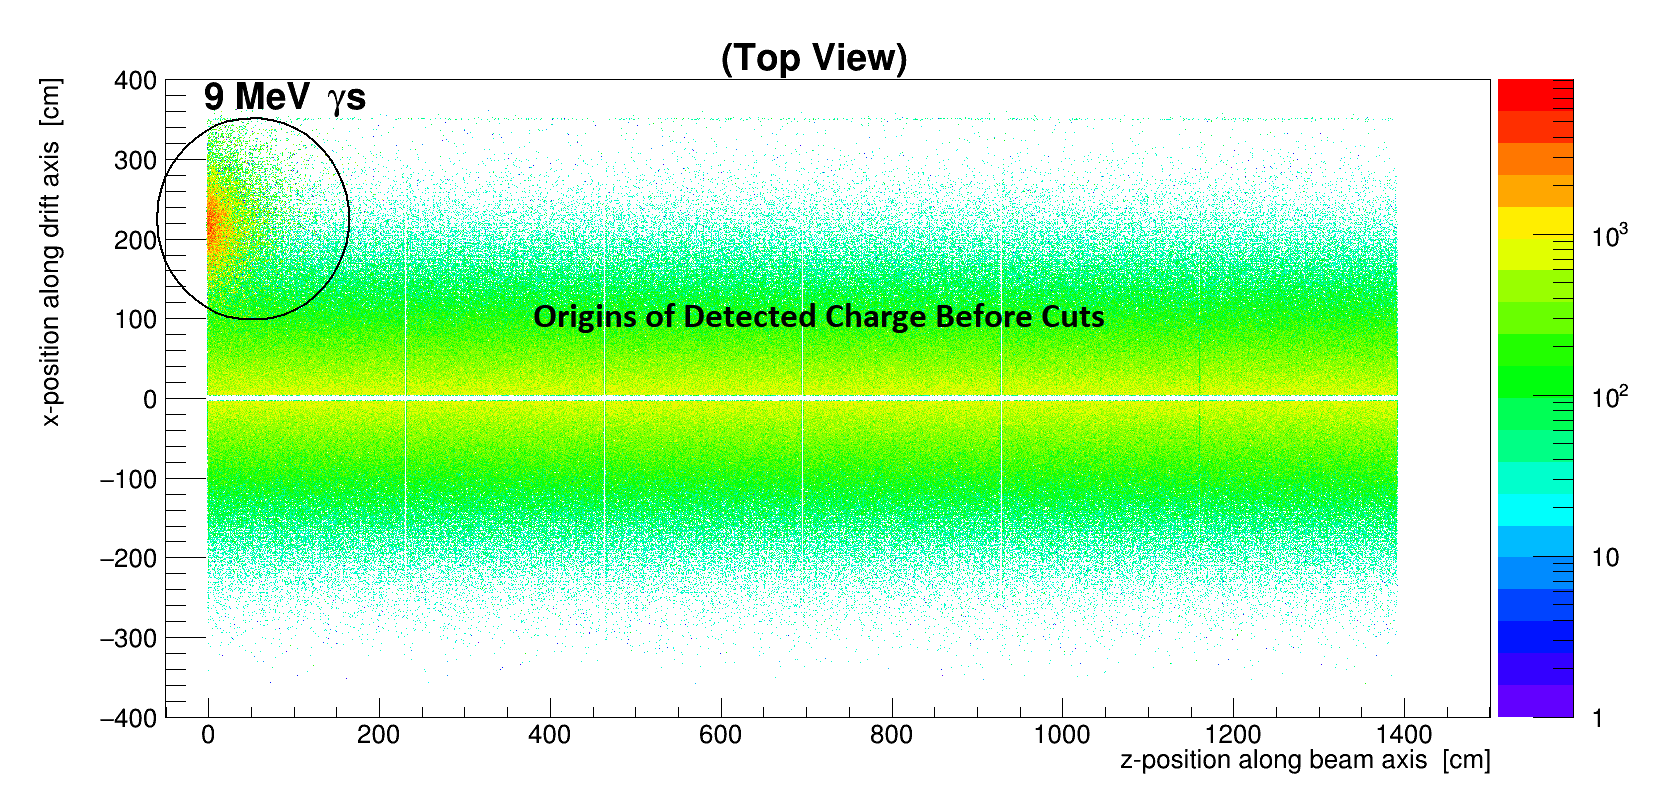
\includegraphics[width=0.76\linewidth]{9MeVgamma_withBG_LArSoft_v08_14_00_hiLY_originCHARGEcollected_TopView_TDR.png}
   (b)
   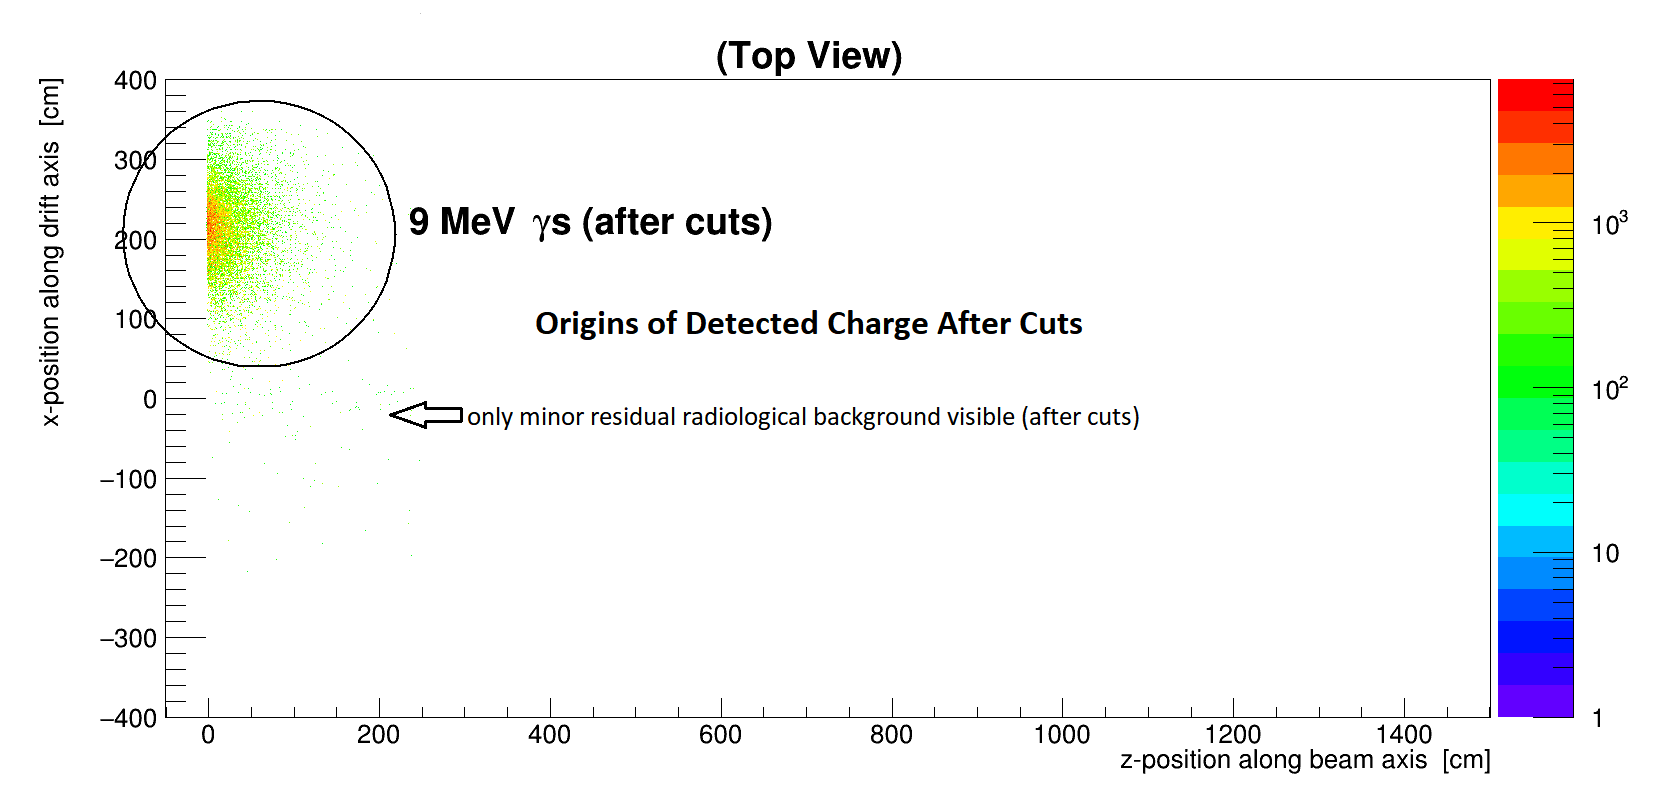
\includegraphics[width=0.75\linewidth]{9MeVgamma_withBG_LArSoft_v08_14_00_hiLY_originCHARGEcollected_TopView_cut_TDR.png}

%    \subfigure[a]{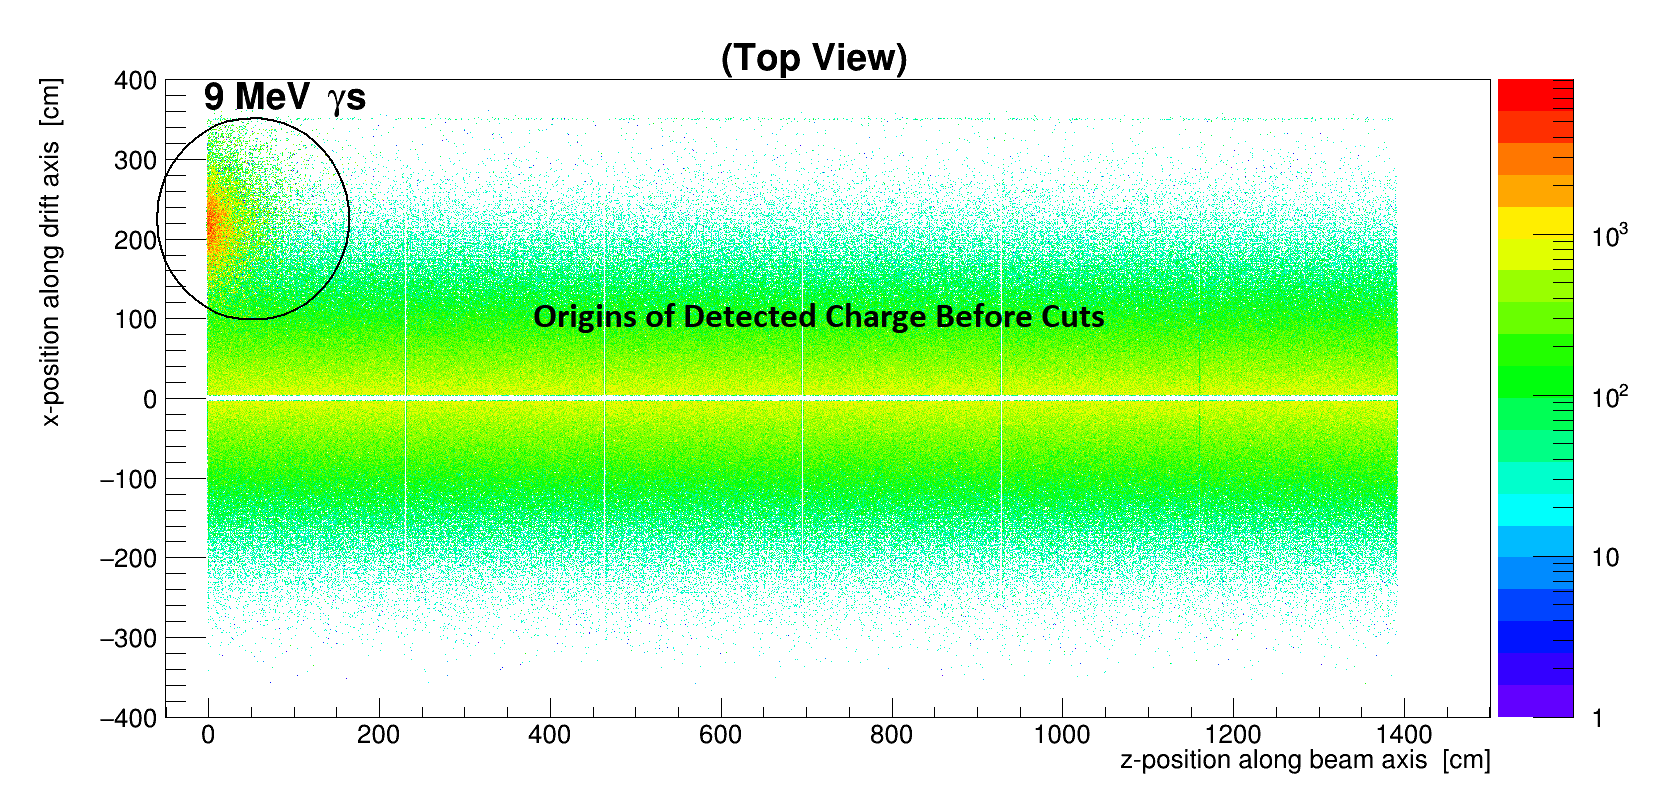
\includegraphics[width=1.0\linewidth]{9MeVgamma_withBG_LArSoft_v08_14_00_hiLY_originCHARGEcollected_TopView_TDR.png}}
%    \subfigure[b]{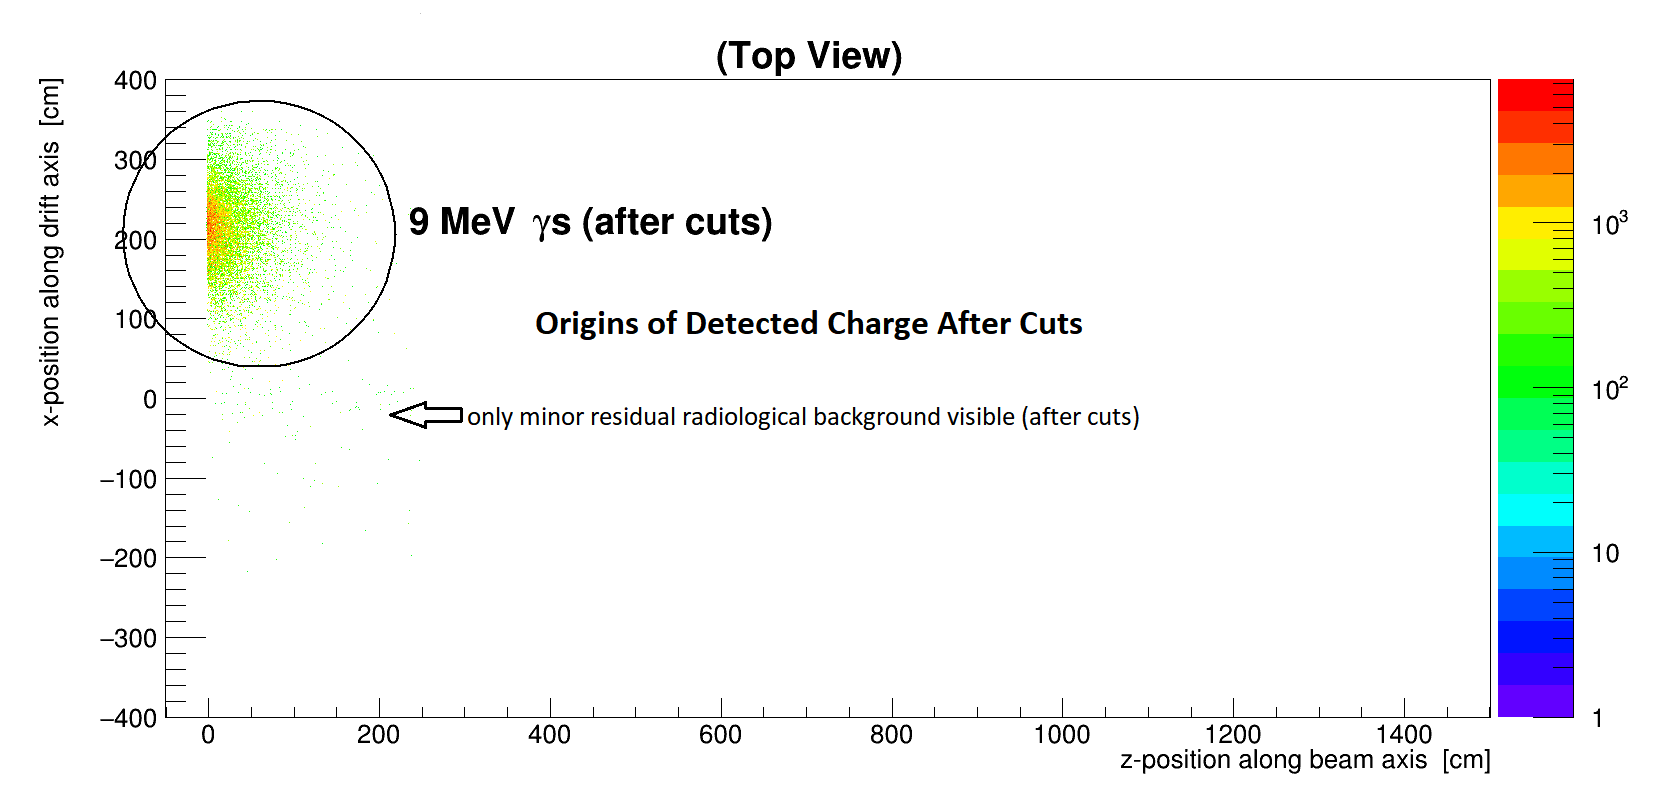
\includegraphics[width=1.0\linewidth]{9MeVgamma_withBG_LArSoft_v08_14_00_hiLY_originCHARGEcollected_TopView_cut_TDR.png}}
\end{dunefigure}

\begin{dunefigure}[Measured \efield and e$^-$ lifetime from \SI{9}{MeV} gamma; with radiological backgrounds]
{fig:rsds-fig2}
%{fig:9MeVgamma_withBG_LArSoft_v08_14_00_hiLY_DriftTimesEfield_ChargeSpectrumElectronLifetime_cut}
{Simulated measurements of (a) \efield strength from drift-time distribution, (b) electron lifetime from drift-time distribution, and (c) electron lifetime from charge distribution when electric field is unambiguously known from drift-time distribution. All spectra were created with applied selection cuts for a simulated \SI{9}{\MeV} $\gamma$-ray source with radiological backgrounds deployed at $z=$\SI{-40}{\cm} outside of the \dword{fc}, $x=$\SI{220}{\cm} away from the \dword{apa}, and $y=$\SI{300}{\cm} half-height of an upper endwall \dword{apa}. (Colors of histograms are matching colors of corresponding labels in each histogram.)}
\centering
    %(a)
    %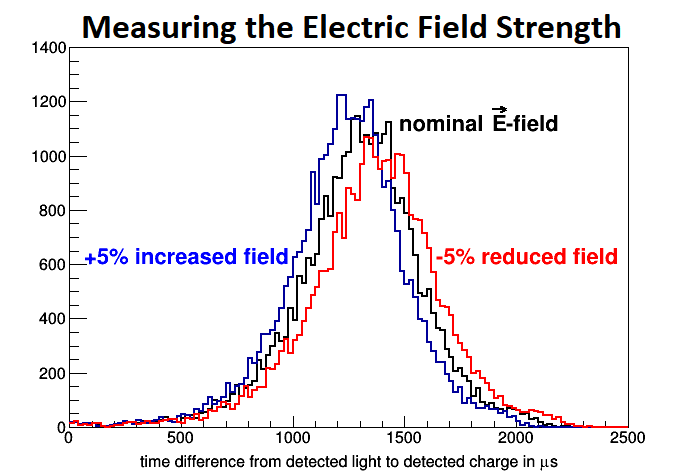
\includegraphics[width=0.45\linewidth]{9MeVgamma_withBG_LArSoft_v08_14_00_hiLY_EfieldDriftTimes_cut_TDR.png}
    %(b)
    %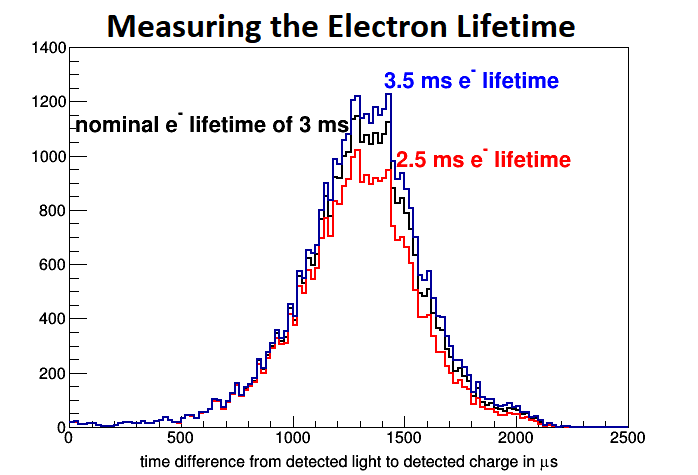
\includegraphics[width=0.45\linewidth]{9MeVgamma_withBG_LArSoft_v08_14_00_hiLY_eLifeTimeDriftTimes_cut_TDR.png}
    %(c)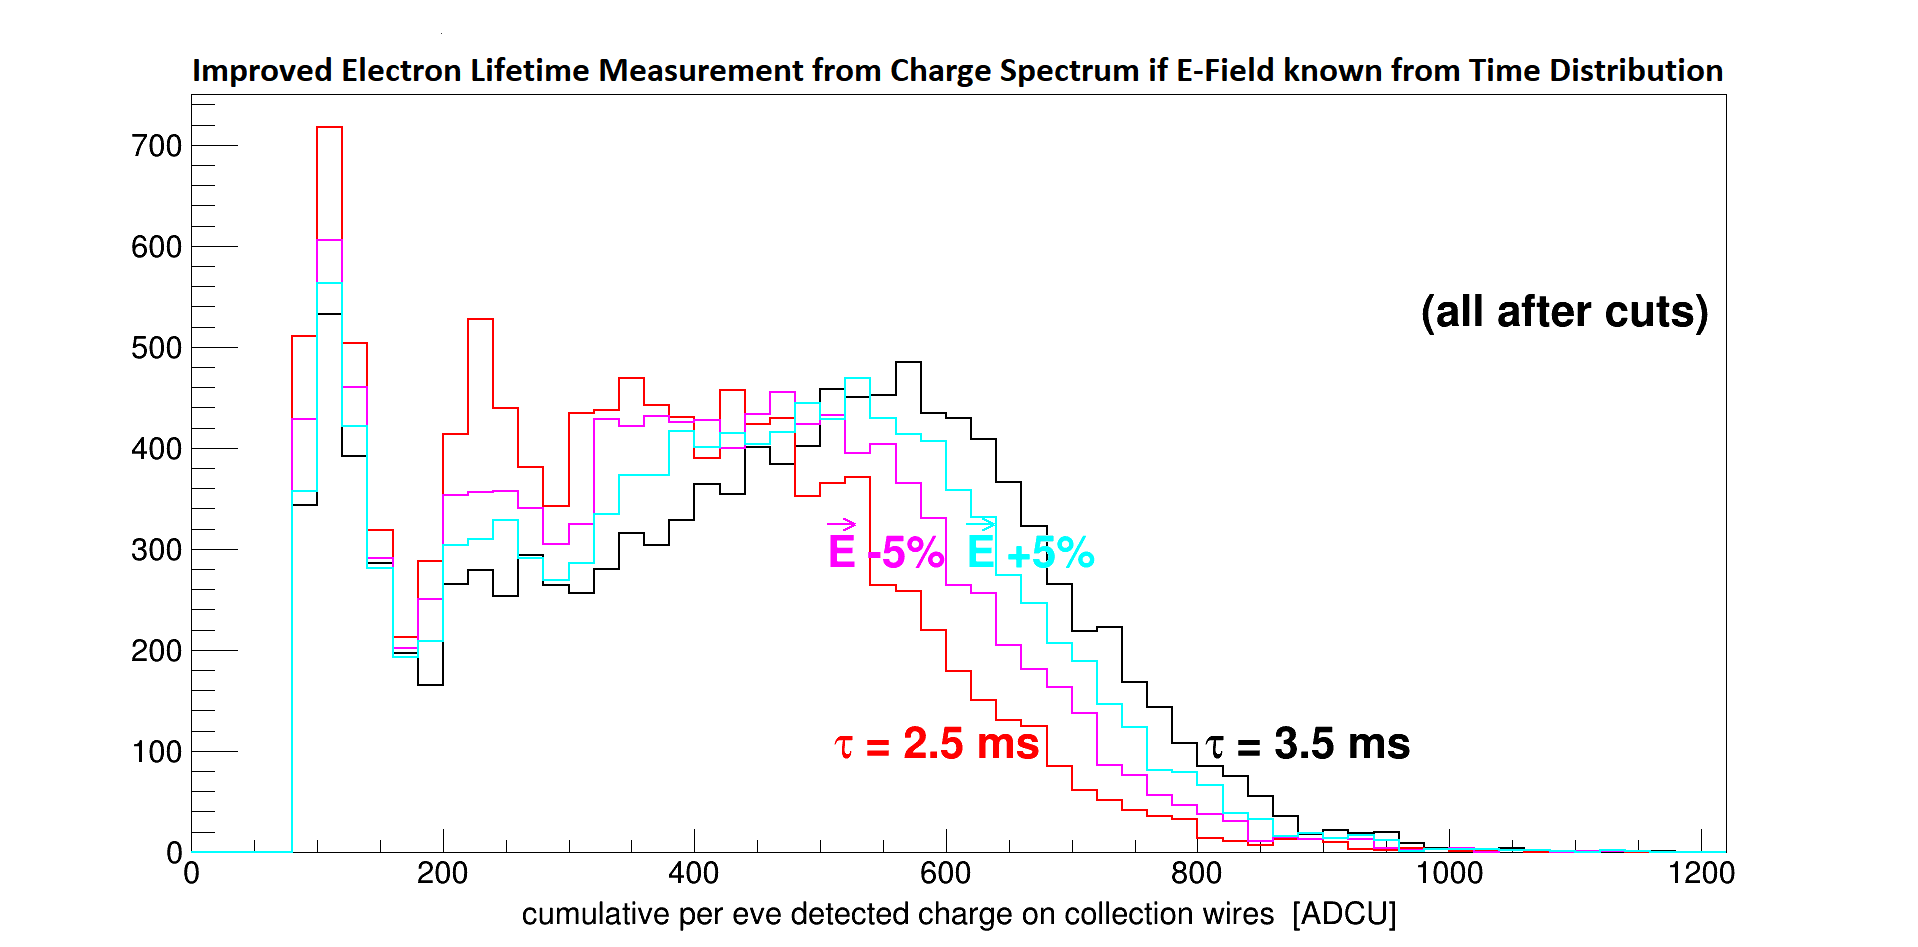
\includegraphics[width=0.75\linewidth]{9MeVgamma_withBG_LArSoft_v08_14_00_hiLY_chargeSpectrum_eLifeTimeEfield_cut_TDR.png}

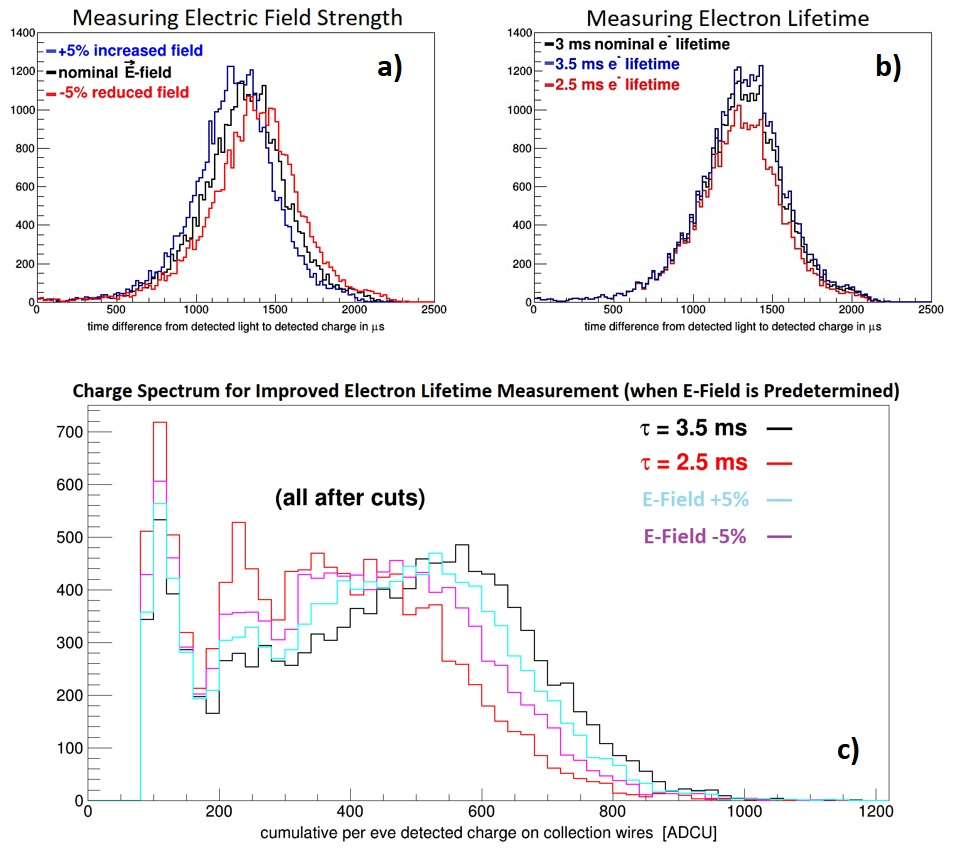
\includegraphics[width=0.9\linewidth]{graphics/9MeVgamma_withBG_EfieldDriftTimes_eLifetime_chargeSpectrum_cut_nicer2.jpg}    
    
%        \subfigure[a]{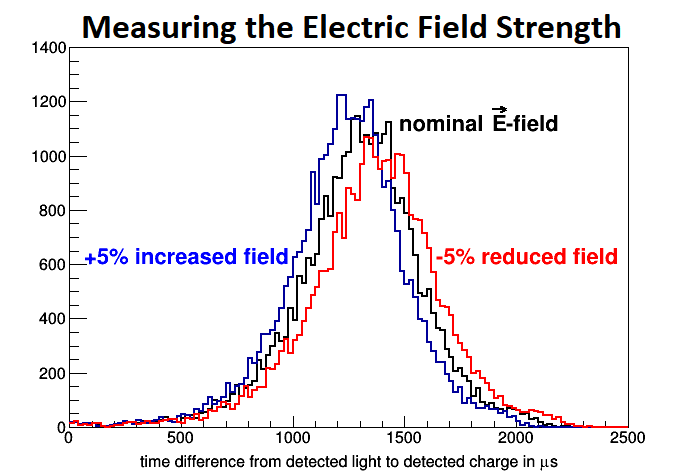
\includegraphics[width=0.45\linewidth]{9MeVgamma_withBG_LArSoft_v08_14_00_hiLY_EfieldDriftTimes_cut_TDR.png}}
%    \subfigure[b]{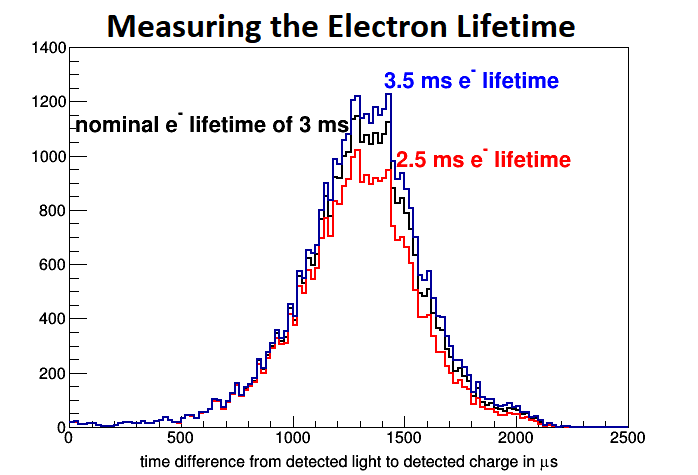
\includegraphics[width=0.45\linewidth]{9MeVgamma_withBG_LArSoft_v08_14_00_hiLY_eLifeTimeDriftTimes_cut_TDR.png}}
%    \subfigure[c]{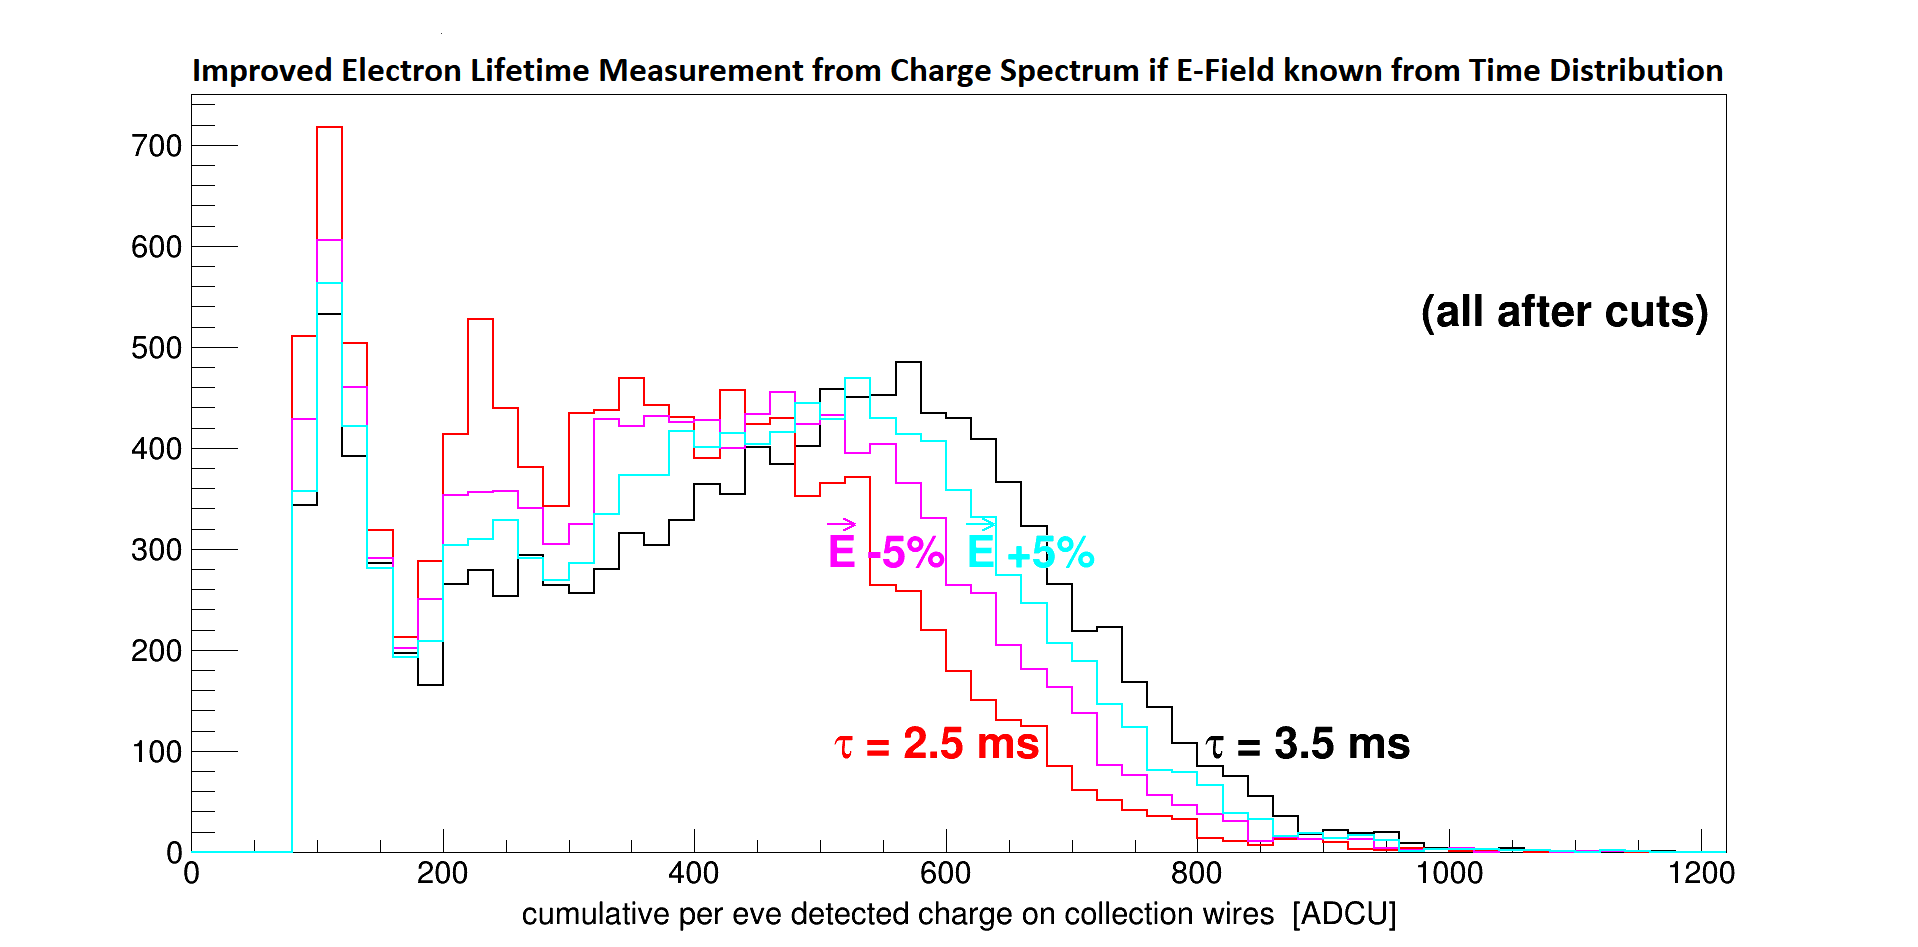
\includegraphics[width=1.0\linewidth]{9MeVgamma_withBG_LArSoft_v08_14_00_hiLY_chargeSpectrum_eLifeTimeEfield_cut_TDR.png}}
\end{dunefigure}

%\begin{dunefigure}[Frequency of optical channel hits with gamma source;  with radiological backgrounds]
%{fig:rsds-fig2plus}
%{fig:5MeValphaSource_zx_TDR_TopView}
%{In LArSoft simulated change in frequency of optical channel hits with a simulated 9~MeV $\gamma$-ray source deployed at $z=$\SI{-40}{\cm} outside of the \dword{fc}, $x=$\SI{220}{\cm} away from the \dword{apa}, and $y=$\SI{300}{\cm} half-height of an upper endwall \dword{apa} with simulated expected radiological background.}
%  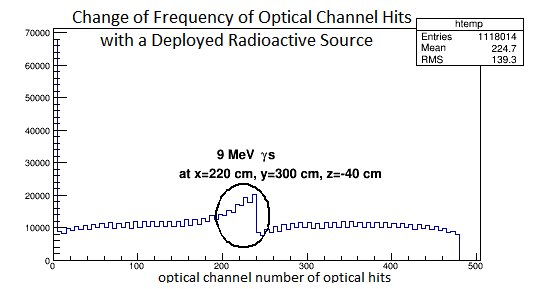
\includegraphics[width=0.6\linewidth]{ophit_opchannels_9MeVgammaSource_wBGs_LArSoft_v08_14_00_geo_v4_TDR.png}
%\end{dunefigure}


%\begin{dunefigure}[Detected light, charge from \SI{15}{MeV} gamma source; no radiological backgrounds]
%{fig:rsds-fig3}
%{fig:5MeValphaSource_zx_TDR_TopView}
%{In LArSoft backtracked origins of detected (a) photoelectrons and (b) charge for a simulated $^{40}$Ar($\alpha,\,\gamma$)$^{44}$Ca 15~MeV $\gamma$-ray source deployed at $z=$\SI{-40}{\cm} outside of the \dword{fc}, $x=$\SI{220}{\cm} away from the \dword{apa}, and $y=$\SI{300}{\cm} half-height of an upper endwall \dword{apa} without simulated expected radiological background.}
%\centering
%   (a)
%   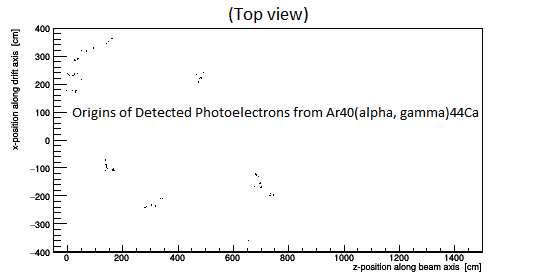
\includegraphics[width=0.455\linewidth]{5MeValphaSource_zx_pe_TDR.png}
%   (b)
%   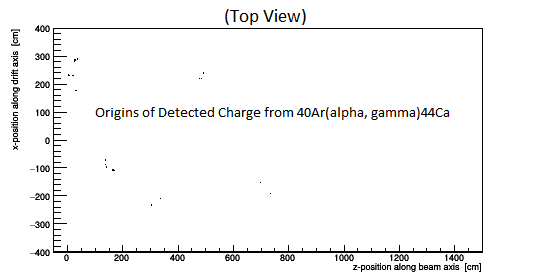
\includegraphics[width=0.455\linewidth]{5MeValphaSource_zx_adc_TDR.png}
%\end{dunefigure}



\subsubsection{\dword{rsds} Design Validation}
%\dword{protodune} forms the ultimate test to validate the design, operation and performance of the system. 
The cosmic induced background rate at \dword{protodune} is too high at the surface to detect responses to the \dword{dune} $\gamma$-ray source; a higher intensity source could be deployed to test the detector response and analysis method. However, tests of functionality,  reliability, and safety of the mechanical deployment system are essential to show the source can be deployed and retrieved with no issues, so these will be the main goals of the \dword{protodune2} deployment. As mentioned earlier, tests of the source design itself, in terms of $\gamma$ activity, will be done at SDSMT. 

\subsubsection{DAQ Requirements}
Section~\ref{sec:sp-calib-daqreq} provides an overall discussion of the Calibration and \dword{daq} interface. Here, the \dword{daq} requirements for the \dlong{rsds} are discussed. The radioactive source will not be triggerable by the \dword{mlt}.  Rather, it will deliver a tag to the \dword{mlt} and that tag will include a time stamp that can be used by the \dword{mlt} to issue a trigger command to the \dword{fe} readout.  The trigger command will have a standard readout window size of \SI{5.4}{\milli\s}, but to keep data rates manageable, the command will only be send to \dword{fe} readout buffers that are expected to be illuminated by the source. The localization of trigger commands thus reduces the data volume by \num{150}, if only one \dword{apa} is read out.

Nevertheless, if the rate of such a source is anywhere close to one per \SI{5.4}{\milli\s}, the detector would be running  continuously in the current scheme. Therefore we assume that the interaction rate in the detector is \SI{10}{\hertz} or less. The tag from the source will likely be much higher than this, because not all $\gamma$s interact in the active \dword{tpc} volume. Thus the radioactive source trigger will be a coincidence in the Module-Level Trigger between a low-energy trigger candidate from the illuminated \dword{apa}, and a source tag with a relevant time stamp.  With this rate, and with localization of events to one \dword{apa}, the total data volume would be

\begin{equation}
\num{8}~{\rm hours} \times \num{4}~{\rm FTs} \times \SI{10}{\hertz} \times \num{1.5}~{\rm Bytes}\times \SI{2}{\mega\hertz}\times \SI{5.4}{\milli\s}\times \num{2560}~{\rm channels} = \SI{50}{\TB}/scan.
\end{equation}

Running this calibration four times/year would yield \SI{200}{\TB} of data in \SI{10}{\kt} per year. Table~\ref{tab:calib-daq-rsds} summarizes the data volume requirements for \dword{rsds}.

\begin{dunetable}
[Calibration \dshort{daq} summary for \dshort{rsds}]
{p{0.2\textwidth}p{0.15\textwidth}p{0.5\textwidth}}
{tab:calib-daq-rsds}
{Estimated data volume per year per \SI{10}{\kt} for the radioactive source system.}   
System & Data Volume (\SI{}{\TB\per\year}) & Assumptions  \\ \toprowrule
Proposed Radioactive Source System & \num{200} & Source rate < \SI{10}{\hertz}; single \dword{apa} readout,  lossless readout; \num{4} times/year   \\ 
\end{dunetable}           

\subsubsection{Risks}
The risks associated with the radioactive source system are described in Table~\ref{tab:risks:SP-FD-CAL-RSDS} along with appropriate mitigation strategies and the impact (low, medium or high risk levels) on probability, cost, and schedule post-mitigation. There are three residual medium-level risks in the table, more discussion on them is provided below:
\begin{itemize}
    \item {\it Radioactivity leak:} If radioactivity leaks into the detector during a deployment, radiological backgrounds in the detector might increase. Rigorous source certification under high pressure and cryogenic temperatures mitigates this risk.
    \item {\it Source stuck or lost:} If the source gets stuck or is lost in the detector, then it becomes a permanent localized radiological background source. Fish-line an order of magnitude stronger than needed to hold the weight, round edges of the moderator and a torque limit of the stepper motor will mitigate this risk.
    \item {\it Oxygen and nitrogen contamination:} If the purge-box has a small leak, oxygen and nitrogen could get into the \dword{lar}. Leak checks before deployments will mitigate this risk.
\end{itemize}


% risk table values for subsystem SP-FD-CAL-RSDS
\begin{footnotesize}
%\begin{longtable}{p{0.18\textwidth}p{0.20\textwidth}p{0.32\textwidth}p{0.02\textwidth}p{0.02\textwidth}p{0.02\textwidth}}
\begin{longtable}{P{0.18\textwidth}P{0.20\textwidth}P{0.32\textwidth}P{0.02\textwidth}P{0.02\textwidth}P{0.02\textwidth}} 
\caption[Risks for SP-FD-CAL-RSDS]{Risks for SP-FD-CAL-RSDS (P=probability, C=cost, S=schedule) More information at \dshort{riskprob}. \fixmehl{ref \texttt{tab:risks:SP-FD-CAL-RSDS}}} \\
\rowcolor{dunesky}
ID & Risk & Mitigation & P & C & S  \\  \colhline
RT-SP-CAL-10 & Radioactive source swings into detector elements & Constrain the system with guide-wires & L & L & L \\  \colhline
RT-SP-CAL-11 & Radioactivity leak & Obtain rigorous source certification under high pressure and cryogenic temperatures & L & L & M \\  \colhline
RT-SP-CAL-12 & Source stuck or lost & Safe engineering margins, stronger fish-line and a torque limit in deployment system & L & M & L \\  \colhline
RT-SP-CAL-13 & Oxygen and nitrogen contamination & Leak checks before deployments & L & M & M \\  \colhline
RT-SP-CAL-14 & Light leak into the detector through purge-box & Light-tight purge box with an infrared camera for visual checks & L & L & L \\  \colhline
RT-SP-CAL-15 & Activation of the cryostat insulation & Activation studies and simulations & L & L & L \\  \colhline

\label{tab:risks:SP-FD-CAL-RSDS}
\end{longtable}
\end{footnotesize}


\begin{comment}
%SG: Old table of risks for RSDS.
\begin{dunetable}
[Calibration risks3]
{p{0.03\linewidth}p{0.4\linewidth}p{0.05\linewidth}p{0.4\linewidth}}
{tab:fdgen-calib-risks3}
{Possible risk scenarios for the radioactive source system along with mitigation strategies. The level of risk is indicated by letters ``H'', ``M'', and ``L'' corresponding to high, medium and low level risks.}   
No. & Risk  & Risk Level & Mitigation Strategy  \\ \toprowrule

10 & The deployed radioactive source can potentially swing into detector elements if not controlled or if large currents exist in the \dword{lar} & M & Guide-wires mitigate this risk.\\ \colhline

11 & Radioactivity could leak into the detector during a deployment. & L & Rigorous source certification under large pressure and cryogenic temperatures mitigates this risk.\\ \colhline

12 & The source could get stuck or lost in the detector. & L & Fish-line an order of magnitude stronger than needed to hold the weight, round edges of the moderator and a torque limit of the stepper motor will mitigate this risk.\\ \colhline

13 & Oxygen and nitrogen could get into the \dword{lar} in case the purge-box has a small leak. & M & Leak checks before deployments, purge-box in under-pressure inside w/r to the detector, will mitigate this risk.\\ \colhline

14 & Light could couple into the detector. & M &
Light-tight purge-box, internally equipped with an infra-red camera for visual checks will mitigate this risk.\\ \colhline

15 & The source activity can activate the cryostat insulation. & L & Detailed simulations/activation measurements can say what is a tolerable activity and the source activity can be chosen to be below that. \\ 
\end{dunetable}
\end{comment}

\subsubsection{Installation, Integration, and Commissioning}
The first elements of the radioactive source guide system are installed before the \dword{tpc} elements on the end wall farthest from the \dword{tco} and as the last system, concurrent and coordinated with the alternative laser system (if any deployed), once the \dword{tpc} is installed before closing the \dword{tco}. The radioactive source deployment system is installed at the top of the cryostat and can be installed when \dword{dune} becomes operational.

The commissioning plan for the source deployment system will include a dummy source deployment (within \num{2} months of the commissioning) followed by first real source deployment (within \num{3} to \num{4} months of the commissioning) and a second real source deployment (within \num{6} months of the commissioning). Assuming stable detector conditions, the radioactive source will be deployed every half a year. Ideally, a deployment before and after a run period are desired so at least two data points are available for calibration. This also provides a check if the state of the system
has changed before and after the physics data run.
%If stability fluctuates for any reason (e.g., electronic response changes over time) at a particular location, one would want to deploy the source at that location once a month, or more often, depending on how bad the stability is.
It is estimated that it will take a few hours (e.g. \num{8}~hours) to deploy the system at one feedthrough location and a full radioactive source calibration campaign might take %at least 
a week.

%\newpage
\subsubsection{Quality Control}
A mechanical test of the Double Chooz fish-line deployment system with a \dword{lar} mock-up column will be done in the high bay laboratory at SDSMT. The ultimate test of the system will be done at \dword{protodune}. Safety checks will also be done for the source and for appropriate storage on the surface and underground. 

\subsubsection{Safety}
\label{sec:sp-calib-rsds-safety}
A composite source is used for the radioactive source system that consists  of \isotope{Cf}{252}, a strong neutron emitter, and \isotope{Ni}{58}, which, via the \isotope{Ni}{58}(n,$\gamma$)\isotope{Ni}{59} process, converts one of the \isotope{Cf}{252} fission neutrons, suitably moderated, to a monoenergetic \SI{9}{\MeV} gamma. This system also poses a radiation risk, which will be mitigated with a purge-box for handling, and a shielded storage box and an area with lockout-tagout procedures, also applied to the gate-valve on top of the cryostat. Material safety data sheets will be submitted to DUNE ES\&H and specific procedures will be developed for storage and handling of sources to meet Fermilab Radiological Control Manual (FRCM) requirements. These procedures will be reviewed and approved by \dword{surf} and \fnal radiation safety officers. Sources that get deployed will be checked monthly to ensure they are not leaking. A designated shielded storage area will be assigned for sources and proper handling procedures will be reviewed periodically. A custodian will be assigned to each shielded source.